\documentclass[12pt]{article}
\usepackage[a4paper,left=3cm,right=2cm,top=2.5cm,bottom=2.5cm]{geometry}
\usepackage{graphicx}
\usepackage{subcaption}
\usepackage[hyphens]{url}
\usepackage{hyperref}



%opening
\title{Kickstarting Application Development\\ with Enterprise Java\\ A Spring Boot Case Study}
\author{Lennart Cockx\\Guangming Luo}

\begin{document}

\maketitle
\newpage
\tableofcontents
\newpage

\begin{abstract}
\noindent In this report we will explore various Java technologies and analyse what features they offer. The focus of this project is to find which frameworks are most suitable for quick prototyping of a business application.
Constraints and other requirements will be defined and will then be applied to a specific case study.
\end{abstract}

\section{Project Objective}
\subsection{Proposal}
This master thesis is commissioned by Faros, a Cronos group company specialized in the development of Java web applications and primarily focused on designing Rich Internet Applications. Development within Faros is done mainly with Vaadin, Spring, HTML5, ExtJS, JavaScript, JSP, JSF, NoSQL and more. This means that during this thesis, special attention is given to these technologies in regards to design choices. Naturally, comparisons with other possible frameworks will still be done and valid arguments will be set forward to confirm these decisions.
\\\\
The following case study was proposed by Faros: designing an online cash register that can be used in restaurants or at events. Existing cash register systems are expensive and for smaller establishments or temporary events, this investment is not worth it. The idea is to use existing devices from employees and customers to handle the ordering and payment process.
\\\\
This project is an opportunity for us to learn about the frameworks and technologies used for the development of rich, interactive web applications. Additionally, we want to explore the best methods to quickly build a web application from scratch. Some key aspects that we will look out for are: Documentation availability, speed of new project setup, customizability, integration with other frameworks and security features. When given the corresponding documentation, it should be possible to reproduce this application. During the design and development of this project we want to describe the problems we faced and how we solved them. This will give other students the option to learn from our mistakes and hopefully help them increase their understanding of Java EE concepts. 
\subsection{Concept}
At the start of the project we discuss the key aspects of this project with our coaches at Faros. Based on the requirements provided by them, combined with our own interests, we will define the general field we will be working in. 
\\\\
After we have a good overview of what aspects must be included in this project (or should be avoided), we can start deciding core features that will determine which technologies will be appropriate for this project. These choices are based on the aspects we think are needed for developing a web application based on the aforementioned requirements. This should give us a list of possible systems and frameworks that could potentially be used during this project.
\\\\
Now that we have a list of possible systems, we can start to think about the case study we want to develop. Once we know the general outline of the project, we can begin selecting the the appropriate tools and frameworks that fit this case study. This will shorten the list to technologies specifically applicable to this project. For certain frameworks it will be difficult to obtain a shorter list, as they might all comply with the requirements we set. In this case we will make a selection of items to keep the scope of the project realistic. Usually the most popular frameworks will be selected. If a deviating set is chosen this will be elaborated on in the corresponding chapter.
\\\\
Now that the tools are known, the standard procedure for application development will be followed. Relevant documentation will be constructed including a use case analysis, feature description (Nice-to-have versus Must-have), navigational models, hierarchical task analysis, UML diagrams and market research. After this we can start working on getting familiar with the chosen enterprise Java frameworks.
\\\\
As soon as we are sufficiently proficient with our chosen tools, we will start working on a case study where we use the knowledge we obtained to build a functional prototype for a realistic use case scenario. During the project we might come to the conclusion that certain choices we made were suboptimal or simply do not allow further progression. In such cases, we will adjust our trajectory and change to the appropriate tools. Any time such a decision is made we will mention it in this report and provide the matching argumentation as to why we made the switch.
\subsection{Project Requirements}
\subsubsection{Constraints}

\subsubsection{Design focus}

\section{Enterprise Java Research}
\subsection{Current Landscape}
\subsection{Comparison of technologies}
\subsubsection{General framework}
\subsubsection{Persistence providers}
\subsubsection{Security}
\subsubsection{Front-end and Styling}
\section{Case study: Online cash register}
\subsection{Introduction}
The goal of this case study is to create a service that can be used at events and in restaurants to process orders made by customers, relay these orders to the waiters and chefs and handle the payment. This service should include an application that clients can use to view the menu and order items from it. Waiters also have their own application that can place and acknowledge orders. These orders will be send to a central system that manages all the required information. See fig. \ref{fig:usecase} for a use case diagram.
\subsection{Use Cases}
In this case study we can identify several distinct actors that will interact differently with the application.
\paragraph{Customer}
The customer is the primary user of this application. They access the menu of a specified restaurant or event. They can place orders, either via the application itself or from a waiter with their own device. Finally, they can pay for the orders that they placed. Again, either via the application or a waiter.
\paragraph{Waiter}
Like the customers, the waiter can access the menu of their restaurant and place orders for their clients. In addition to this they can display an overview of the currently queued orders, with the corresponding table numbers or location. They will also handle payments from customers through the application, or accept payment in other forms of currency.
\paragraph{Chef}
The chef can access similar functions as the waiter. Additionally, they can modify the status of an order and mark it as completed or in progress.
\paragraph{Manager}
The manager can modify the menu and change prices. They can also create accounts for employees and give them the corresponding privileges.\\

%should also have some information about multi-tenancy
\begin{figure}[h!]
	\centering
	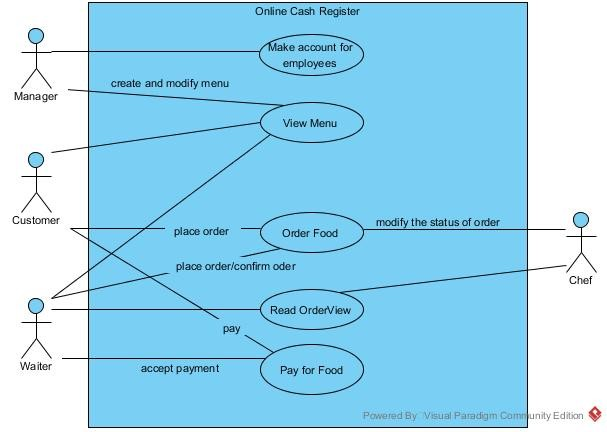
\includegraphics[width=0.75\linewidth]{usecase.jpg}
	\caption{Use Case Diagram}
	\label{fig:usecase}
\end{figure}

\subsection{Must-haves and nice-to haves}
As soon as we had the use cases defined, we can specify what features are absolutely essential and which are optional. This was done in collaboration with our coaches at Faros and gave us the following specifications.
\paragraph{Must-Haves}
\begin{itemize}
	\item The system can be used by multiple managers or event-organizers simultaneously. 
	(\textit{Multi-tenancy})
	\item A central application will handle orders and payment. 
	(\textit{Central application})
	\item Waiters can use an application to send the orders of customers to the kitchen and accept payment. 
	(\textit{Employee interface + Payment system})
	\item Customers can view the menu of the restaurant/event with their mobile device. 
	(\textit{Customer interface})
	\item An order overview is available for the waiters and chefs. It shows the completed orders and orders which have to be made. 
	(\textit{Order overview})
	\item Customers can add comments to certain items. E.g. no tomato
	(\textit{Special requests}) 
	\item Customers can place their own orders with their mobile device. 
	(\textit{Customer Mobile ordering})
	\item Prevent customers from making ridiculous orders or misusing the system.
	(\textit{Misuse prevention})
\end{itemize}
\paragraph{Nice-to-Haves}
\begin{itemize}
	\item Event organizers can run the central application on their own local network. 
	(\textit{Local network hosting})
	\item After an order is finished, the completed order number is shown on a big screen. 
	(\textit{Take-a-number/Now serving System})
	\item The manager can find statistics on his restaurant and orders via a web app. 
	(\textit{Order Statistic}s)
	\item Customers can split the bill or combine orders 
	(\textit{Bill splitting})
	\item Provide an easy way for customers to use our system at an event/restaurant. Even if they don’t know it yet. 
	(\textit{Easy access})
	\item Customers can order additional food or drinks. This will be added to the total bill.
	(\textit{Multiple orders})
	
\end{itemize}

\subsection{Technology choices}
\subsubsection{Application type}
\subsubsection{Framework choices}
\subsection{Design Choices}
\subsubsection{Client}
%Possibly insert pictures we designed
%This part will need to be reviewed as changes to the design were made
We want to make an application for customers of restaurants and events. The customer can use this application to get an overview of the available menu items and prices. If the customers have decided, they can order the desired dishes straight from the application. Finally, the customers can pay for their meal with this application.
We can differentiate a couple of different scenarios when the customer goes to a restaurant or event that supports this system. We assume that a web app is used. If a native or hybrid application is used, installing the app will be an additional step before using the system.
\\\\
After (or before) the meal is finished, customers should be able to pay directly from within the application or pay a waiter. When using the application to place an order for multiple people, the customers should have the option to order and pay separately or order together and split the cost. 
For example: Three people want to place an order, two of which have access to the application. 
\begin{itemize}
\item One person can place the order for the entire group.
\item One person can order for himself and the person without the application. While the third person makes his own choice with his own device.
\item The two persons with the application order for themselves, while the other person orders something from a waiter.
\end{itemize}

\noindent 
In all three cases the order will be combined into one order for that table. After the meal the bill can be paid for.

\begin{itemize}
	\item One person decides to pay for the entire bill. This can be paid to a waiter or with his application.
	\item Each person pays for the part he ordered separately, with the price corresponding to what they ordered.
	\item Everyone decides to split up the bill equally, dividing the total cost over three people. 
\end{itemize}

\noindent
Typically, when people eat at a restaurant, they will place multiple orders. During the meal additional drinks might be ordered and at the end of the meal some people might want a dessert or coffee. We have to design the application so it can accept multiple orders and display the sum of these orders at the end of the meal.


\subsubsection{Employee}
To be able to interact with customers using this system, the waiters and chefs will need their own version of this application. They will need to get an overview of the current orders placed and they should be able to modify and confirm these orders.
\\\\
The order overview will have all the relevant information of the order: The different dishes and drinks ordered by the customer, the table from which the order was placed, the price and the status of the order. Additional information such as a time and date and an order number can be added for statistical purposes.
The order overview could look something like this:
\begin{figure}[h!]
	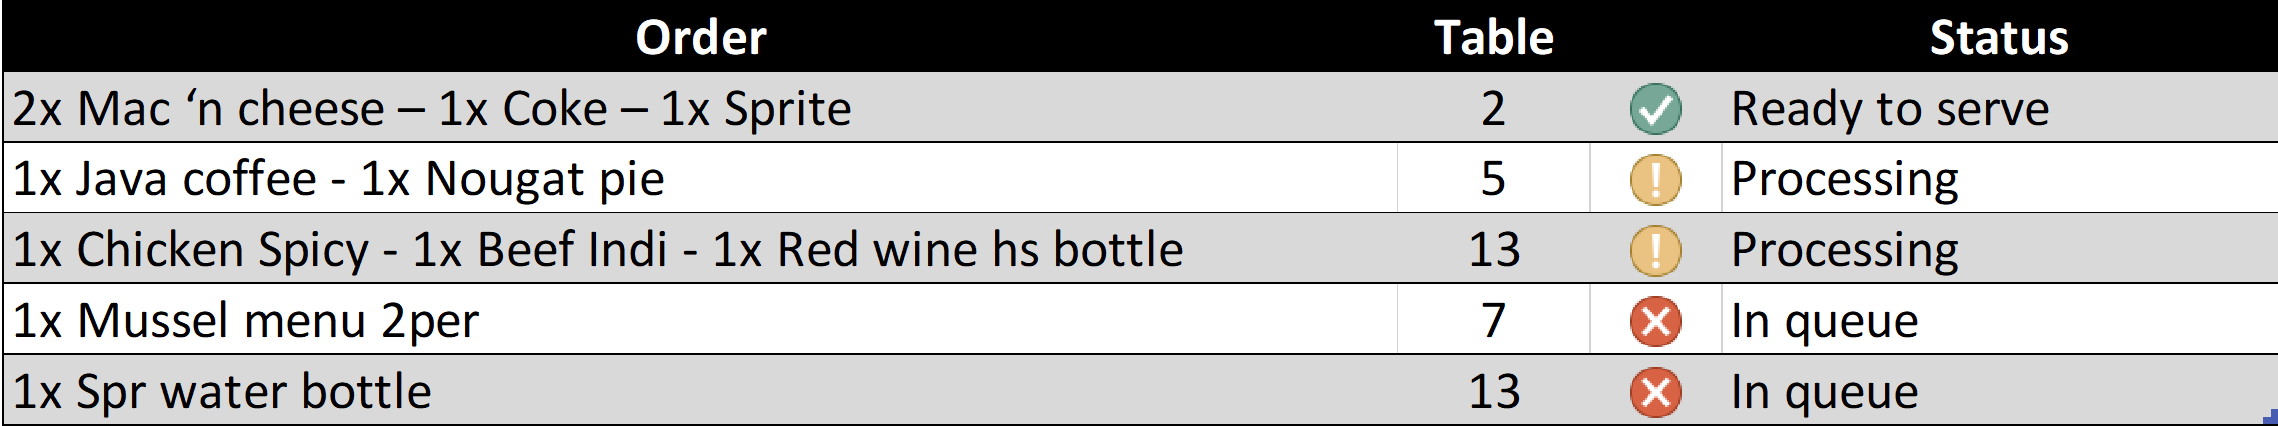
\includegraphics[width=\linewidth]{orderview.PNG}
	\caption{Example Order Overview}
	\label{fig:orderview}
\end{figure}
\\
Whenever an order is served, it will be removed from the overview and the next item will be moved up. When the bill is requested, all orders from the corresponding table will be added together. After payment the orders for that table are reset to allow the next customers to place their order.
\\\\
In some cases, an order might be wrong or a mistake with the number of dishes is made. The application should be flexible and allow a waiter to make small modifications to the order to correct a mistake.
Additionally, a customer might make a special request for his order. This can be due to allergies or plainly because of a certain preference. It might be useful to provide a bit of space to the order overview for extra remarks.
\\\\
An order might contain a lot of different items. The full names of these items will take a lot of space in the order overview. Typically, a shorthand notation is used by waiters to more efficiently note down and read orders. A similar system could be used for the order overview.
Also, for showing the menu to the customer we will display a vertical list with the name of every menu item. This list will contain detailed information like the name of the dish, the ingredients, pricing and possibly even a picture. These menu items can be sorted into categories for easy navigation. On the other side, the waiter does not need all the detailed information. Instead a compact and efficient layout is preferred to be able to easily take an order. This could be a grid layout with simple icons or abbreviations for each dish. See fig. \ref{fig:waitercustomer}.
\begin{figure}[h!]
	\begin{subfigure}{.5\textwidth}
		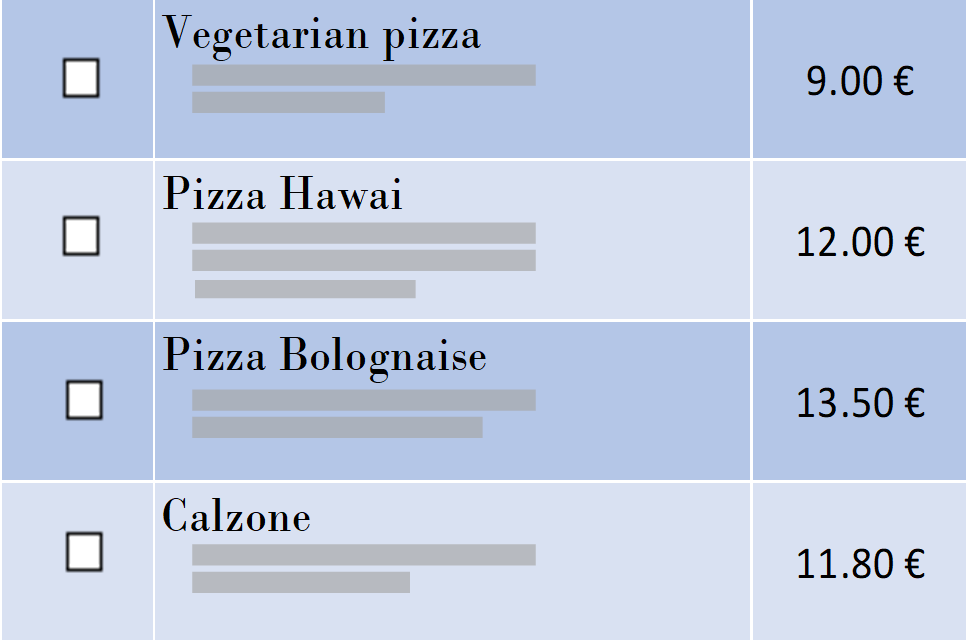
\includegraphics[width=0.9\linewidth]{customermenu.PNG}
		\caption{Customer Menu Layout}
		\label{fig:menucustomer}
	\end{subfigure}
	\begin{subfigure}{.5\textwidth}
		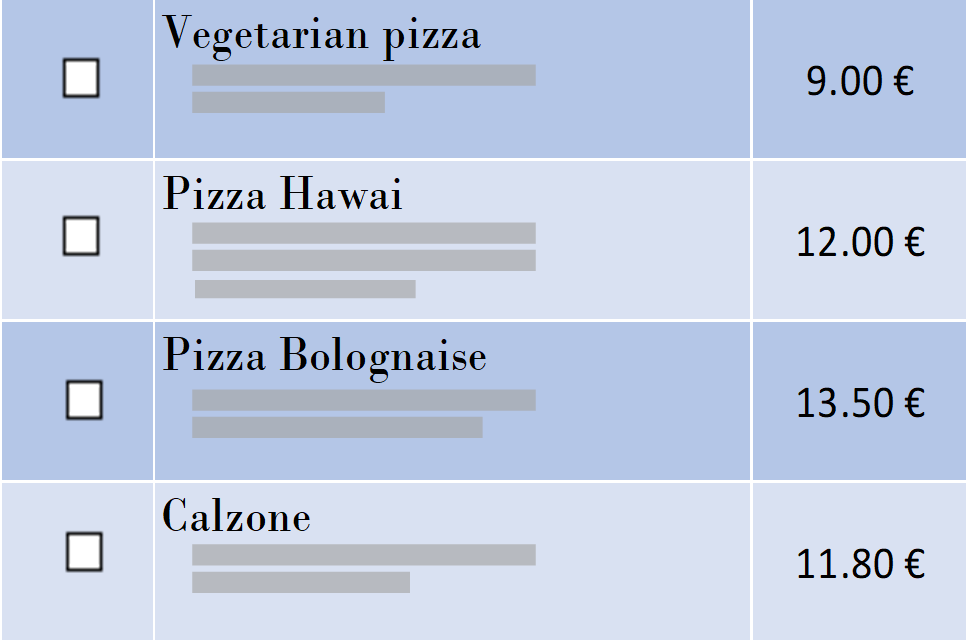
\includegraphics[width=0.9\linewidth]{customermenu.PNG}
		\caption{Waiter Menu Layout}
		\label{fig:waitercustomer}
	\end{subfigure}
	\caption{Menu Layouts}
	\label{fig:menus}
\end{figure}

\noindent \\It is possible that certain people with bad intent might try to place orders for ridiculous amounts of food, repeatedly place small orders to fill the system or even place orders for another table. Some of these situations can be prevented with proper programming like limiting the amount of orders one table can make each minute. Another way to prevent some of these issues is to have waiters confirm orders on their device before adding them to the kitchen. In day to day use, these scenarios will be rare, but it’s still important to think about the possible problems that might occur. 
While a user account for the customer might be desirable to track certain statistics and prevent misuse of the system (like mentioned above), requiring an account might not be interesting, as this can make the process of using the application slow and unintuitive for the customer.


\subsubsection{Manager}
\subsubsection{Remarks and challenges}
\subsection{Major issues and their solutions}




blablabla \cite{greenwade93} \cite{antonov2015spring} \cite{JavaTool10:online} \cite{farosProposal} \cite{SpringPopular1:online}


\newpage
\bibliographystyle{plain}
\bibliography{document}

\end{document}
